%%%%%%%%%%%%%%%%%%%%%%%%%%%%%%%%%%%%%%%%%%%%%%%%%%%%%%%%%%%%%%%%%%%%%%%%%%%%%%%
% Análisis en una variable
%
% Copyright (c) 2016 Damián Silvestre. Permission is granted to copy, 
% distribute and/or modify this document under the terms of the 
% GNU Free Documentation License, Version 1.3 or any later version published by
% the Free Software Foundation; with no Invariant Sections, no 
% Front-Cover Texts, and no Back-Cover Texts. 
%
% Details of the GNU FDL can be found here: 
% http://www.gnu.org/licenses/licenses.html
%
%%%%%%%%%%%%%%%%%%%%%%%%%%%%%%%%%%%%%%%%%%%%%%%%%%%%%%%%%%%%%%%%%%%%%%%%%%%%%%%

\part{Análisis en una variable}

%%%%%%%%%%%%%%%%%%%%%%%%%%%%%%%%%%%%%%%%%%%%%%%%%%%%%%%%%%%%%5
\chapter{Topología en la recta real}

\section{Recta real}

Recordar las propiedades que definen al conjunto de los números reales (ver \ref{numeros_reales}), que también llamaremos recta real por su representación gráfica.

\begin{figure}[h]
\centering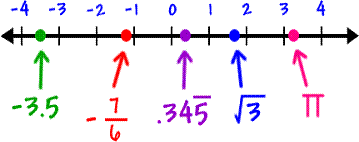
\includegraphics[scale=0.6]{images/03_analisis1/number_line.png}
\caption{Recta real}
\end{figure}

\begin{definition}[Entorno] \label{entorno_real}
Dados $x_0 \in \RR$ y $r > 0$ 
	
Llamamos \textbf{entorno} \index{Recta real!Entorno} (o entorno abierto) de centro $x_0$ y radio $r$ al conjunto
	
$$ E(x_0,r) = \{ x \in \RR^n : d(x,x_0) < r\} $$
	
Llamamos \textbf{entorno cerrado} de centro $x_0$ y radio $r$ al conjunto
	
$$ E[x_0,r] = \{ x \in \RR^n : d(x,x_0) \leq r\} $$
	
Llamamos \textbf{entorno reducido} de centro $x_0$ y radio $r$ a 
	
$$ E'(x_0,r) = E(x_0,r) - \{x_0\}$$
\end{definition}


\begin{definition}[Puntos] \label{clasif_topo_puntos_r}
	
Sea $A \subseteq \RR$, y $x \in \RR$, entonces decimos que $x$ respecto de $A$ es 
	
\begin{itemize}
\item \textbf{Punto interior}: Si existe $E(x,\delta) \subseteq A$.
		
\item \textbf{Punto exterior}: Si existe $E(x,\delta) \subseteq \RR^n - A$.  Equivalentemente $E(x,\delta) \cap A = \emptyset$.
		
\item \textbf{Punto frontera}: Si no es punto interior ni exterior.  Es decir que para todo $ \delta > 0$ se tiene $E(x,\delta) \cap A \neq \emptyset$ y $E(x,\delta) \cap (\RR - A) \neq \emptyset$
		
\item \textbf{Punto clausura} (o adherencia): Si existe un entorno tal que $E(x,r) \cap A \neq \emptyset$
		
\item \textbf{Punto de acumulación} (o punto límite): Si para todo entorno del punto, $ E(x,r) \cap (A - \{x\}) \neq \emptyset$.
		
Equivalentemente, si para todo entorno reducido del punto, $ E'(x,r) \cap A \neq \emptyset$
		
\item \textbf{Punto aislado}: Si existe un entorno tal que $E(x,r) \cap A = \{x\}$
\end{itemize}
\end{definition}

\begin{definition}[Interior] \label{conjunto_interior_r}
Sea $A \subseteq \RR$.  Entonces definimos
	
El \textbf{interior de $A$} como el conjunto de sus puntos interiores, lo denotamos $A^{\circ}$
	
La \textbf{clausura de $A$} como el conjunto de sus puntos de clausura, lo denotamos $\overline{A}$
	
El \textbf{conjunto derivado de $A$} como el conjunto de todos sus puntos de acumulación, lo denotamos $A'$
\end{definition}

%%%%%%%%%%%%%%%%%%%%%%%%%%%%%%%%%%%%%%%%%%%%%%%%%%%%%%%%%%%%%5
\chapter{Límite de funciones reales}

\begin{definition}[Límite] \label{limite_r}
Sea $f : A \subset \RR \to \RR$, $ a \in A'$, y $L \in \RR$.  Se dice que el \textbf{límite de $f$ cuando $x$ tiende a $a$} \index{Continuidad!Límite} es $L$ si se cumple cualquiera que:

Para todo $\epsilon > 0$ existe $\delta > 0$ tal que si $x \in A$, $0 < |x-a| < \delta$ entonces $|f(x) - L| < \epsilon$

y en ese caso escribimos

$$ \displaystyle \lim_{x \to a} f(x) = L $$
\end{definition}

\enazul{Escribir sobre límites laterales, propiedades de límites, infinitésimos equivalentes}

\begin{theorem}[Cero por acotada] \label{cero_por_acotada}
Sean $f,g:A \subseteq \RR \to \RR$, $a \in A'$.

Si $f$ es infinitésimo en $a$ (es decir $ \lim_{x \to a} f(x) = 0$), y $g$ es acotada (es decir $g(A)$ un conjunto acotado) entonces

$$ \lim_{x \to a} f(x)g(x) = 0 $$
\end{theorem}



%%%%%%%%%%%%%%%%%%%%%%%%%%%%%%%%%%%%%%%%%%%%%%%%%%%%%%%%%%%%%5
\chapter{Funciones contínuas}


\begin{theorem}[Bolzano]
Sea $f : A \to \RR$ contínua en $[a,b] \subseteq A$, con $f(a) f(b) < 0$ (es decir tal que $f(a)$ y $f(b)$ tienen signo opuesto).

Entonces existe $c \in [a,b]$ tal que $f(c) = 0$ (es decir existe una raíz)
\end{theorem}









%%%%%%%%%%%%%%%%%%%%%%%%%%%%%%%%%%%%%%%%%%%%%%%%%%%%%%%%%%%%%5
\chapter{Funciones diferenciables}

%%%%%%%%%%%%%%%%%%%%%%%%%%%%%%%%%%%%%%%%%%%%%%%%%%%%%%%%%%%%%5
\chapter{Aproximación de funciones por polinomios}

%%%%%%%%%%%%%%%%%%%%%%%%%%%%%%%%%%%%%%%%%%%%%%%%%%%%%%%%%%%%%5
%\chapter{Integral indefinida}

%%%%%%%%%%%%%%%%%%%%%%%%%%%%%%%%%%%%%%%%%%%%%%%%%%%%%%%%%%%%%5
\chapter{Cálculo integral}

%%%%%%%%%%%%%%%%%%%%%%%%%%%%%%%%%%%%%%%%%%%%%%%%%%%%%%%%%%%%%5
\chapter{Relaciones entre el cálculo diferencial e integral}

%%%%%%%%%%%%%%%%%%%%%%%%%%%%%%%%%%%%%%%%%%%%%%%%%%%%%%%%%%%%%5
\chapter{Sucesiones, series numéricas y funcionales}



